\title{\textbf{Galerkin Attention: Petrov-Galerkin Projection onto Orthonormal Bases for Transformer Self-Attention}}

\author{Anonymous authors}



\section{Introduction}

\subsection{Motivation}

Self-attention computes pairwise interactions between all tokens in a 
sequence, yielding an $N \times N$ attention matrix. This quadratic cost 
in sequence length is the primary bottleneck for long-context transformers. 
A natural question arises: **can attention be reformulated in a lower-dimensional 
space without losing its expressive power?**

One classical approach is to view attention as a discretization of the 
continuous non-local integral operator:

\[
(\mathcal{K} f)(x) = \int_\Omega k(x, y) f(y) \, dy
\]

where $k(x, y)$ is a kernel and $\Omega$ is the domain. Petrov-Galerkin 
methods approximate such operators by projecting onto finite-dimensional 
subspaces:

\[
\mathcal{K} \approx \Phi \, K_{\Phi \Phi} \, \Phi^\top
\]

where $\Phi \in \mathbb{R}^{N \times r}$ is a basis and $K_{\Phi \Phi}$ is 
the projected kernel matrix.

0.85


\subsection{Problem Statement}

Given a pretrained transformer with hidden size $d$ and $H$ heads, we seek 
a modified attention function $\mathcal{A}'$ such that:

\[
\mathcal{A}'(Q, K, V) \approx \mathcal{A}(Q, K, V), \quad
\text{Cost}(\mathcal{A}') = \mathcal{O}(Nr^2), \quad r \ll N
\]

We do not require retraining of base weights; LoRA adapters provide 
recovery capacity.

\subsection{Our Approach}

We propose \textbf{Galerkin Attention}, which:

\begin{enumerate}
\item \textbf{Projects} $Q, K, V$ onto an orthonormal DCT basis $\Phi \in \mathbb{R}^{N \times r}$:
  $$
  Q\_\Phi = \Phi^\top Q, \quad K\_\Phi = \Phi^\top K, \quad V\_\Phi = \Phi^\top V
  $$

\item \textbf{Computes attention} in the reduced basis space:
  $$
  O\_\Phi = \mathrm{softmax}\!\left(\frac{Q\_\Phi K\_\Phi^\top}{\sqrt{d}}\right) V\_\Phi
  $$

\item \textbf{Reconstructs} to the original sequence length:
  $$
  O = \Phi \, O\_\Phi
  $$

\item \textbf{Falls back} to standard causal attention for decoder models.

\end{enumerate}
\subsection{Contributions}

\begin{itemize}
\item \textbf{A Petrov-Galerkin formulation of attention} using fixed DCT basis
  projection.
\item \textbf{An empirical evaluation} on DistilBERT, RoBERTa, and GPT-2 on SST-2.
\item \textbf{A negative result:} encoder models lose 25--30\% accuracy; the method
  fails as a compression technique.
\item \textbf{An analysis} attributing failure to the fixed, data-independent basis.
\item \textbf{Full reproducibility}, including code and checkpoints.

\end{itemize}
\subsection{Paper Organization}

Section 2 reviews related work on Galerkin methods, spectral attention, 
and low-rank attention. Section 3 provides background on attention, DCT, 
and Petrov-Galerkin projection. Section 4 presents Galerkin Attention. 
Section 5 covers architecture integration. Section 6 details the 
experimental setup. Section 7 reports results. Section 8 analyzes why the 
method fails. Section 9 discusses lessons learned. Section 10 lists 
limitations. Section 11 concludes.



\subsection{Notation}

\begin{table}[H]
\centering
\small
\begin{tabular}{lll}
\toprule
\textbf{Symbol} & \textbf{Meaning} & \textbf{First appears} \\
\midrule
$N$ \& Sequence length & 1.1 \\
$d$ \& Head dimension & 1.1 \\
$H$ \& Number of heads & 1.1 \\
$r$ \& Basis dimension (rank) & 1.1 \\
$\Phi \in \mathbb{R}^{N \times r}$ \& Orthonormal basis & 1.1 \\
$\mathcal{K}$ \& Integral operator & 1.1 \\
$k(x, y)$ \& Kernel function & 1.1 \\
$Q_\Phi, K_\Phi, V_\Phi$ \& Basis-projected Q/K/V & 1.3 \\
\bottomrule
\end{tabular}
\end{table}
</parameter>




\section{Related Work}

\subsection{Petrov-Galerkin Methods}

Petrov-Galerkin methods (Quarteroni \& Valli, 1994) approximate solutions of 
differential and integral equations by projecting onto finite-dimensional 
subspaces. Unlike Galerkin methods (test = trial space), Petrov-Galerkin 
uses different test and trial spaces, allowing non-symmetric operators to be 
handled. Our approach uses the same basis for trial and test -- a \textbf{Bubnov-Galerkin} 
variant -- but we retain the "Petrov" terminology following the original 
motivation of the module.

\textbf{Kernel methods.} The Nystr m method (Williams \& Seeger, 2001) also 
approximates kernel matrices via low-rank projection. Our approach differs 
in using a \textbf{fixed basis} rather than sampled landmarks.

\subsection{Spectral Attention}

\textbf{FNet} (Lee-Thorp et al., 2021). Replaces attention entirely with a 2D 
Fourier transform, achieving $\mathcal{O}(N \log N)$ complexity. This is the 
closest work to ours in spirit -- but FNet replaces attention, while we 
project it.

\textbf{Random feature attention} (Peng et al., 2021). Uses random features to 
approximate softmax. Performer (Choromanski et al., 2021) uses positive 
orthogonal random features.

\textbf{Nystr mformer} (Xiong et al., 2021). Uses Nystr m landmarks for low-rank 
attention approximation. Landmarks are data-dependent; our basis is fixed.

\subsection{Low-Rank Attention}

\textbf{Linformer} (Wang et al., 2020). Projects K and V to a lower rank via 
learned linear maps. Our projection is a fixed DCT basis.

\textbf{Synthesizer} (Tay et al., 2021). Uses learned or random attention 
matrices. Random Synthesizer is data-independent like ours.

\subsection{Position of Our Work}

\begin{table}[H]
\centering
\small
\begin{tabular}{lll}
\toprule
\textbf{Axis} & \textbf{Prior work} & \textbf{Galerkin} \\
\midrule
\textbf{Basis type} \& Learned (Linformer) or landmarks (Nystr m) \& Fixed DCT \\
\textbf{Attention replacement} \& Full or partial \& Projection only \\
\textbf{Parameter cost} \& Zero or reduced & \textbf{Added LoRA} \\
\textbf{Encoder support} \& Yes \& Yes (but fails) \\
\textbf{Decoder support} \& Yes \& Falls back \\
\bottomrule
\end{tabular}
\end{table}

\textbf{Key distinction.} Unlike Linformer which \textbf{learns} low-rank projections, 
our approach uses a \textbf{fixed} DCT basis. This eliminates the parameter cost 
of projection matrices but sacrifices adaptivity. Our negative results 
suggest this trade-off is not worth it for attention.



\subsection{Comparison Table}

\begin{table}[H]
\centering
\small
\begin{tabular}{lllll}
\toprule
\textbf{Method} & \textbf{Basis} & \textbf{Learned?} & \textbf{Params} & \textbf{SST-2 (DistilBERT)} \\
\midrule
Standard MHSA & -- & -- & 66.9M & 90.71\% \\
Linformer \& Linear \& Yes \& Similar & ~88\% \\
FNet \& Fourier \& No & 66.9M & ~85\% \\
Random Synthesizer \& Random \& No & 66.9M & ~85\% \\
\textbf{Galerkin} & \textbf{DCT} & \textbf{No} & \textbf{+0.9\%} & \textbf{50.92\%} \\
\bottomrule
\end{tabular}
\end{table}




\section{Background}

\subsection{Scaled Dot-Product Attention}

For input $X \in \mathbb{R}^{B \times N \times d}$, attention computes:

\[
\text{Attn}(Q, K, V) = \text{softmax}\!\left(\frac{QK^\top}{\sqrt{d}}\right) V
\]

where $Q = XW_Q$, $K = XW_K$, $V = XW_V$.

\textbf{Cost.} Time and memory for $QK^\top$ are $\mathcal{O}(N^2)$.

\subsection{Discrete Cosine Transform (DCT)}

The DCT-II basis is defined as:

\[
\Phi_{n, k} = \cos\!\left(\frac{\pi k (2n + 1)}{2N}\right), \quad
n = 0, \dots, N-1, \quad k = 0, \dots, N-1
\]

with normalization:

\[
\Phi_{n, 0} \to \frac{1}{\sqrt{N}} \Phi_{n, 0}, \quad
\Phi_{n, k} \to \sqrt{\frac{2}{N}} \Phi_{n, k} \text{ for } k \geq 1
\]

The full DCT basis $\Phi \in \mathbb{R}^{N \times N}$ is orthonormal: 
$\Phi^\top \Phi = I_N$.

\textbf{Why DCT?} DCT is optimal for energy compaction of smooth signals 
(Ahmed et al., 1974). For smooth attention kernels, DCT projection preserves 
most energy.

\textbf{Truncation.} Keeping only the first $r$ columns gives 
$\Phi_r \in \mathbb{R}^{N \times r}$, which satisfies 
$\Phi_r^\top \Phi_r = I_r$.

\subsection{Petrov-Galerkin Projection}

Consider the continuous integral operator:

\[
(\mathcal{K} f)(x) = \int_0^1 k(x, y) f(y) \, dy
\]

Let $\{\phi_1, \dots, \phi_r\}$ be an orthonormal basis of a subspace 
$\mathcal{V}_r \subset L^2([0, 1])$. The Galerkin approximation is:

\[
\mathcal{K}_r = \sum_{i, j = 1}^r K_{ij} \phi_i \otimes \phi_j
\]

where $K_{ij} = \langle \phi_i, \mathcal{K} \phi_j \rangle$.

\textbf{Discretization.} For a discrete sequence of length $N$, the Galerkin 
approximation becomes:

\[
\mathcal{K}_r = \Phi_r \, K_r \, \Phi_r^\top, \quad
K_r \in \mathbb{R}^{r \times r}
\]

with $\Phi_r \in \mathbb{R}^{N \times r}$ being the discrete basis.

\subsection{LoRA Recovery}

After replacing attention, we freeze base weights and train LoRA adapters:

\[
\Delta W = \frac{\alpha}{r_L} B A
\]

with $A \in \mathbb{R}^{r_L \times k}$, $B \in \mathbb{R}^{d \times r_L}$, 
$B = 0$ at init.

\subsection{Notation Summary}

\begin{table}[H]
\centering
\small
\begin{tabular}{ll}
\toprule
\textbf{Symbol} & \textbf{Meaning} \\
\midrule
$B$ \& Batch size \\
$N$ \& Sequence length \\
$d$ \& Hidden dimension \\
$H$ \& Number of heads \\
$r$ \& Basis dimension \\
$\Phi$ \& Orthonormal basis ($N \times r$) \\
$\Phi_r$ \& Truncated basis \\
$r_L$ \& LoRA rank \\
$\mathcal{K}$ \& Integral operator \\
$k(x, y)$ \& Kernel function \\
\bottomrule
\end{tabular}
\end{table}




\section{Method}

\subsection{Overview}

Galerkin Attention has two paths:

\begin{enumerate}
\item \textbf{Encoder path} (bidirectional models): project attention onto DCT basis.
\item \textbf{Decoder path} (causal models): fall back to standard causal attention.

\end{enumerate}
\begin{lstlisting}
                    Input X
                       |
                        
                 +-----------+
                 |  Q/K/V    |
                 | projection|
                 +-----+-----+
                       |
                        
                 +-----------+
                 | is_decoder|
                 +--+----+---+
                    | No | Yes
                    |    |
                    |     
                    |  +--------------+
                    |  | Causal       |
                    |  | attention    |
                    |  | (standard)   |
                    |  +------+-------+
                    |         |
                              |
            +---------------+ |
            | Galerkin proj | |
            | + softmax     | |
            +-------+-------+ |
                    |         |
                    +----+----+
                         |
                          
                    Output Y
\end{lstlisting}

\subsection{The Galerkin Basis}

We construct the DCT-II basis $\Phi \in \mathbb{R}^{N \times r}$:

\[
\Phi_{n, k} = \cos\!\left(\frac{\pi k (2n + 1)}{2N}\right) \cdot
c_k, \quad c_k = \begin{cases} 1/\sqrt{N} \& k = 0 \\ \sqrt{2/N} \& k \geq 1 \end{cases}
\]

We then orthonormalize via QR to correct for numerical error:

\[
\Phi \leftarrow Q \text{ where } \Phi + 10^{-4} I = Q R
\]

\subsection{Projection and Attention}

For each head:

\begin{enumerate}
\item \textbf{Project} Q, K, V onto the basis:
  \[
Q\_\Phi = \Phi^\top Q \in \mathbb{R}^{B \times H \times r \times d}
\]
  
\item \textbf{Compute attention} in the reduced space:
  \[
A\_\Phi = \mathrm{softmax}\!\left(\frac{Q\_\Phi K\_\Phi^\top}{\sqrt{d}}\right) \in \mathbb{R}^{B \times H \times r \times r}
\]
  
\item \textbf{Apply to values:}
  \[
O\_\Phi = A\_\Phi V\_\Phi \in \mathbb{R}^{B \times H \times r \times d}
\]
  
\item \textbf{Reconstruct} to original space:
  \[
O = \Phi O\_\Phi \in \mathbb{R}^{B \times H \times N \times d}
\]

\item \textbf{Energy correction:}
  \[
O \leftarrow O \cdot \sqrt{N / r}
\]

\end{enumerate}
\subsection{Why the Energy Correction?}

The projection $\Phi^\top$ is contractive: $\|\Phi^\top Q\|_F \leq \|Q\|_F$. 
For an orthonormal basis of $r$ columns out of $N$, the average energy 
preserved is $r/N$. Multiplying by $\sqrt{N/r}$ approximately restores 
the original norm.

\textbf{Caveat.} This correction is a heuristic and does not account for the 
actual distribution of energy across the basis. If energy is concentrated 
in the first $r$ components, the correction \textbf{overshoots}; if it is 
uniform, the correction is exact.

\subsection{Decoder Fallback}

For causal models, we use standard attention with explicit causal masking:

\[
\text{scores}_{ij} = \begin{cases}
Q_i K_j^\top / \sqrt{d} \& j \leq i \\
-\infty \& j > i
\end{cases}
\]

This preserves the autoregressive property. The Galerkin path is \textbf{not} 
used for decoders.

\subsection{Parameter Analysis}

Galerkin Attention \textbf{adds parameters} via LoRA:

\begin{table}[H]
\centering
\small
\begin{tabular}{ll}
\toprule
\textbf{Component} & \textbf{Params} \\
\midrule
Original attention & $d_\text{in} d_\text{out}$ \\
Q projection + LoRA & $d_\text{in} d_\text{out} + r_L(d_\text{in} + d_\text{out})$ \\
K projection + LoRA \& same \\
V projection + LoRA \& same \\
O projection + LoRA \& same \\
\textbf{Total per layer} & $4 d_\text{in} d_\text{out} + 4 r_L(d_\text{in} + d_\text{out})$ \\
\bottomrule
\end{tabular}
\end{table}

\textbf{Example (DistilBERT, $r_L = 16$, $d = 768$):} +589,824 params per layer.

\textbf{Note.} Galerkin Attention is \textbf{not a compression method}. It aims to 
reduce \textbf{attention-matrix memory}, not parameter count.

\subsection{Complexity Analysis}

\begin{table}[H]
\centering
\small
\begin{tabular}{lll}
\toprule
\textbf{Component} & \textbf{Time} & \textbf{Memory} \\
\midrule
Q/K/V proj & $\mathcal{O}(Nd^2)$ & $\mathcal{O}(Nd)$ \\
Basis projection & $\mathcal{O}(Nrd)$ & $\mathcal{O}(Nrd)$ \\
Attention & $\mathcal{O}(r^2 d)$ & $\mathcal{O}(r^2)$ \\
Reconstruction & $\mathcal{O}(Nrd)$ & $\mathcal{O}(Nrd)$ \\
O proj & $\mathcal{O}(Nd^2)$ & $\mathcal{O}(Nd)$ \\
\textbf{Baseline MHSA} & $\mathcal{O}(N^2 d)$ & $\mathcal{O}(N^2)$ \\
\textbf{Galerkin} & $\mathcal{O}(Nrd + r^2 d)$ & $\mathcal{O}(Nr)$ \\
\bottomrule
\end{tabular}
\end{table}

For $r \ll N$, Galerkin attention is asymptotically faster in the 
attention matrix, but the projection/reconstruction overhead dominates 
for short sequences.

\subsection{Algorithm}

\textbf{Algorithm 1:} Galerkin Attention forward
\begin{lstlisting}
Input:  X $\in$ R^{B$\times$N$\times$d}, is_decoder
Output: Y $\in$ R^{B$\times$N$\times$d}

 1: Q $\leftarrow$ X W_Q;  K $\leftarrow$ X W_K;  V $\leftarrow$ X W_V
 2: if RoPE: (Q, K) $\leftarrow$ Rotary(Q, K)
 3: if GQA: (K, V) $\leftarrow$ repeat_kv(K, V)
 4:
 5: if is_decoder:
 6:     A $\leftarrow$ causal_softmax(Q K^T / sqrt(d))
 7:     O $\leftarrow$ A V
 8: else:
 9:       $\leftarrow$ DCT_basis(N, r)                 Orthonormal
10:     Q_  $\leftarrow$  ^T Q
11:     K_  $\leftarrow$  ^T K
12:     V_  $\leftarrow$  ^T V
13:     A_  $\leftarrow$ softmax(Q_  K_ ^T / sqrt(d))
14:     O_  $\leftarrow$ A_  V_ 
15:     O $\leftarrow$   O_ 
16:     O $\leftarrow$ O * sqrt(N / r)                 Energy correction
17:
18: return out_proj(O)
\end{lstlisting}

\subsection{Theoretical Basis}

The method is motivated by the following observation: for smooth attention 
kernels $k(x, y)$, projection onto the first $r$ DCT basis functions 
preserves energy at rate:

\[
\frac{\|\Phi_r^\top k\|_2}{\|k\|_2} \approx 1 - \mathcal{O}(r^{-2\alpha})
\]

where $\alpha$ is the smoothness parameter of $k$. For $C^\infty$ kernels, 
the decay is super-polynomial.

\textbf{Empirical caveat.} Trained transformer attention kernels are \textbf{not} 
smooth. They are sharply peaked (attention sinks, heavy hitters) and highly 
content-dependent. This is why our method fails in practice (Section 8).




\section{Architecture Integration}

\subsection{Model Support Matrix}

\begin{table}[H]
\centering
\small
\begin{tabular}{llllll}
\toprule
\textbf{Architecture} & \textbf{Attention} & \textbf{Nested?} & \textbf{RoPE?} & \textbf{GQA?} & \textbf{Galerkin path?} \\
\midrule
DistilBERT & \texttt{MultiHeadSelfAttention} \& No \& No \& No & (encoder) \\
RoBERTa & \texttt{BertSelfAttention} \& Yes \& No \& No & (encoder) \\
GPT-2 & \texttt{GPT2Attention} \& No \& No \& No & (decoder fallback) \\
Qwen3.5 & \texttt{Qwen3Attention} \& No \& Yes \& Yes & (decoder fallback) \\
\bottomrule
\end{tabular}
\end{table}

\subsection{Weight Transfer}

\subsubsection{Conv1D Orientation (GPT-2)}

HuggingFace \texttt{Conv1D} stores \texttt{(in, out)}; we transpose to \texttt{(out, in)}:

\begin{lstlisting}
if "Conv1D" in cls_c or hasattr(c_attn_mod, "nf"):
    c_w = c_w.t()
\end{lstlisting}

We detect via class name \textbf{or} shape heuristic \texttt{w.shape[0] < w.shape[1]}.

\subsubsection{Nested Encoder Detection (RoBERTa)}

The detection order matters. We check \texttt{out\_lin} \textbf{first}:

\begin{lstlisting}
has_out_lin = hasattr(src, "out_lin") or hasattr(src, "c_proj") or hasattr(src, "o_proj")

if has_out_lin:
    is_nested = False     # DistilBERT has out_lin inside attention
elif (hasattr(src, "self") and hasattr(src.self, "query")
      and hasattr(src, "output") and hasattr(src.output, "dense")):
    is_nested = True      # RoBERTa
elif cls_name in ["BertSelfAttention", "RobertaSelfAttention"]:
    is_nested = True
else:
    is_nested = False
\end{lstlisting}

\textbf{Critical bug avoided.} DistilBERT's \texttt{MultiHeadSelfAttention} ends with 
"SelfAttention" and would be misclassified as nested if we did not check 
\texttt{out\_lin} first.

\subsubsection{GQA Support}

For Qwen with $H_{kv} < H$:

\begin{lstlisting}
if self.num_kv_heads != self.num_heads:
    K = repeat_kv(K, self.kv_repeat)
    V = repeat_kv(V, self.kv_repeat)
\end{lstlisting}

\texttt{repeat\_kv} broadcasts and reshapes:

\begin{lstlisting}
def repeat_kv(x, n_rep):
    B, H_kv, N, d = x.shape
    x = x[:, :, None, :, :].expand(B, H_kv, n_rep, N, d)
    return x.reshape(B, H_kv * n_rep, N, d)
\end{lstlisting}

\subsection{Injection Algorithm}

\textbf{Algorithm 2:} Inject Galerkin Attention
\begin{lstlisting}
Input:  layer  , config, old_attn
Output: new attention in  

 1: new $\leftarrow$ GalerkinAttention(config, old_attn=old_attn)
 2: if copy_weights fails: return None
 3: if   has .attention.self:
 4:      .attention.self $\leftarrow$ new
 5:     new.is_nested_encoder $\leftarrow$ True
 6: elif   has .attention:
 7:      .attention $\leftarrow$ new
 8: elif   has .attn:
 9:      .attn $\leftarrow$ new
10: elif   has .self_attn:
11:      .self_attn $\leftarrow$ new
12: return new
\end{lstlisting}

\subsection{Causal Handling}

The \texttt{is\_decoder} flag determines which path is taken:

\begin{lstlisting}
is_dec = (
    getattr(config, "is_decoder", False)
    or getattr(config, "is_causal", False)
    or any(_mt.startswith(p) for p in ("gpt", "qwen", "llama", "mistral"))
)
\end{lstlisting}

For GPT-2 and Qwen, \texttt{is\_decoder=True} and the fallback path is taken.

\subsection{RoPE Support}

Galerkin Attention handles partial RoPE via dimension slicing:

\begin{lstlisting}
rotary_dim = cos.shape[-1]
if rotary_dim < head_dim:
    q_rot, q_pass = q[..., :rotary_dim], q[..., rotary_dim:]
    q_rot_embed = q_rot * cos + rotate_half(q_rot) * sin
    q = torch.cat([q_rot_embed, q_pass], dim=-1)
\end{lstlisting}

\subsection{Failure Handling}

\begin{table}[H]
\centering
\small
\begin{tabular}{lll}
\toprule
\textbf{Failure} & \textbf{Detection} & \textbf{Response} \\
\midrule
Weight copy failure \& Frobenius < 1e-4 \& Log warning \\
Missing projection & \texttt{missing\_after} non-empty \& Log warning \\
Basis QR failure \& try/except \& Fallback \\
Cross-attention & \texttt{encoder\_hidden\_states != None} \& Not supported \\
\bottomrule
\end{tabular}
\end{table}

\subsection{Registry}

\begin{lstlisting}
@ATTENTION_REGISTRY.register("galerkin")
@ATTENTION_REGISTRY.register("galerkin_attention")
class GalerkinAttention(BaseAttention):
    ...
\end{lstlisting}

\subsection{Common Pitfalls}

\subsubsection{Basis Rebuild per Forward}

The basis $\Phi$ is rebuilt on every forward call because it depends on 
$N = $ sequence length. For a fixed $N$, this is wasteful. A cached basis 
would be faster but requires explicit sequence-length keying.

\subsubsection{Fixed Basis Cannot Adapt}

The DCT basis is data-independent. It cannot learn to attend to specific 
positions or content. This is the root cause of the negative results.

\subsubsection{Nested Encoder Double-Projection}

If \texttt{is\_nested\_encoder} is wrong, the output projection is applied twice 
(once inside our module, once by the outer block).



\begin{figure}[H]
\centering
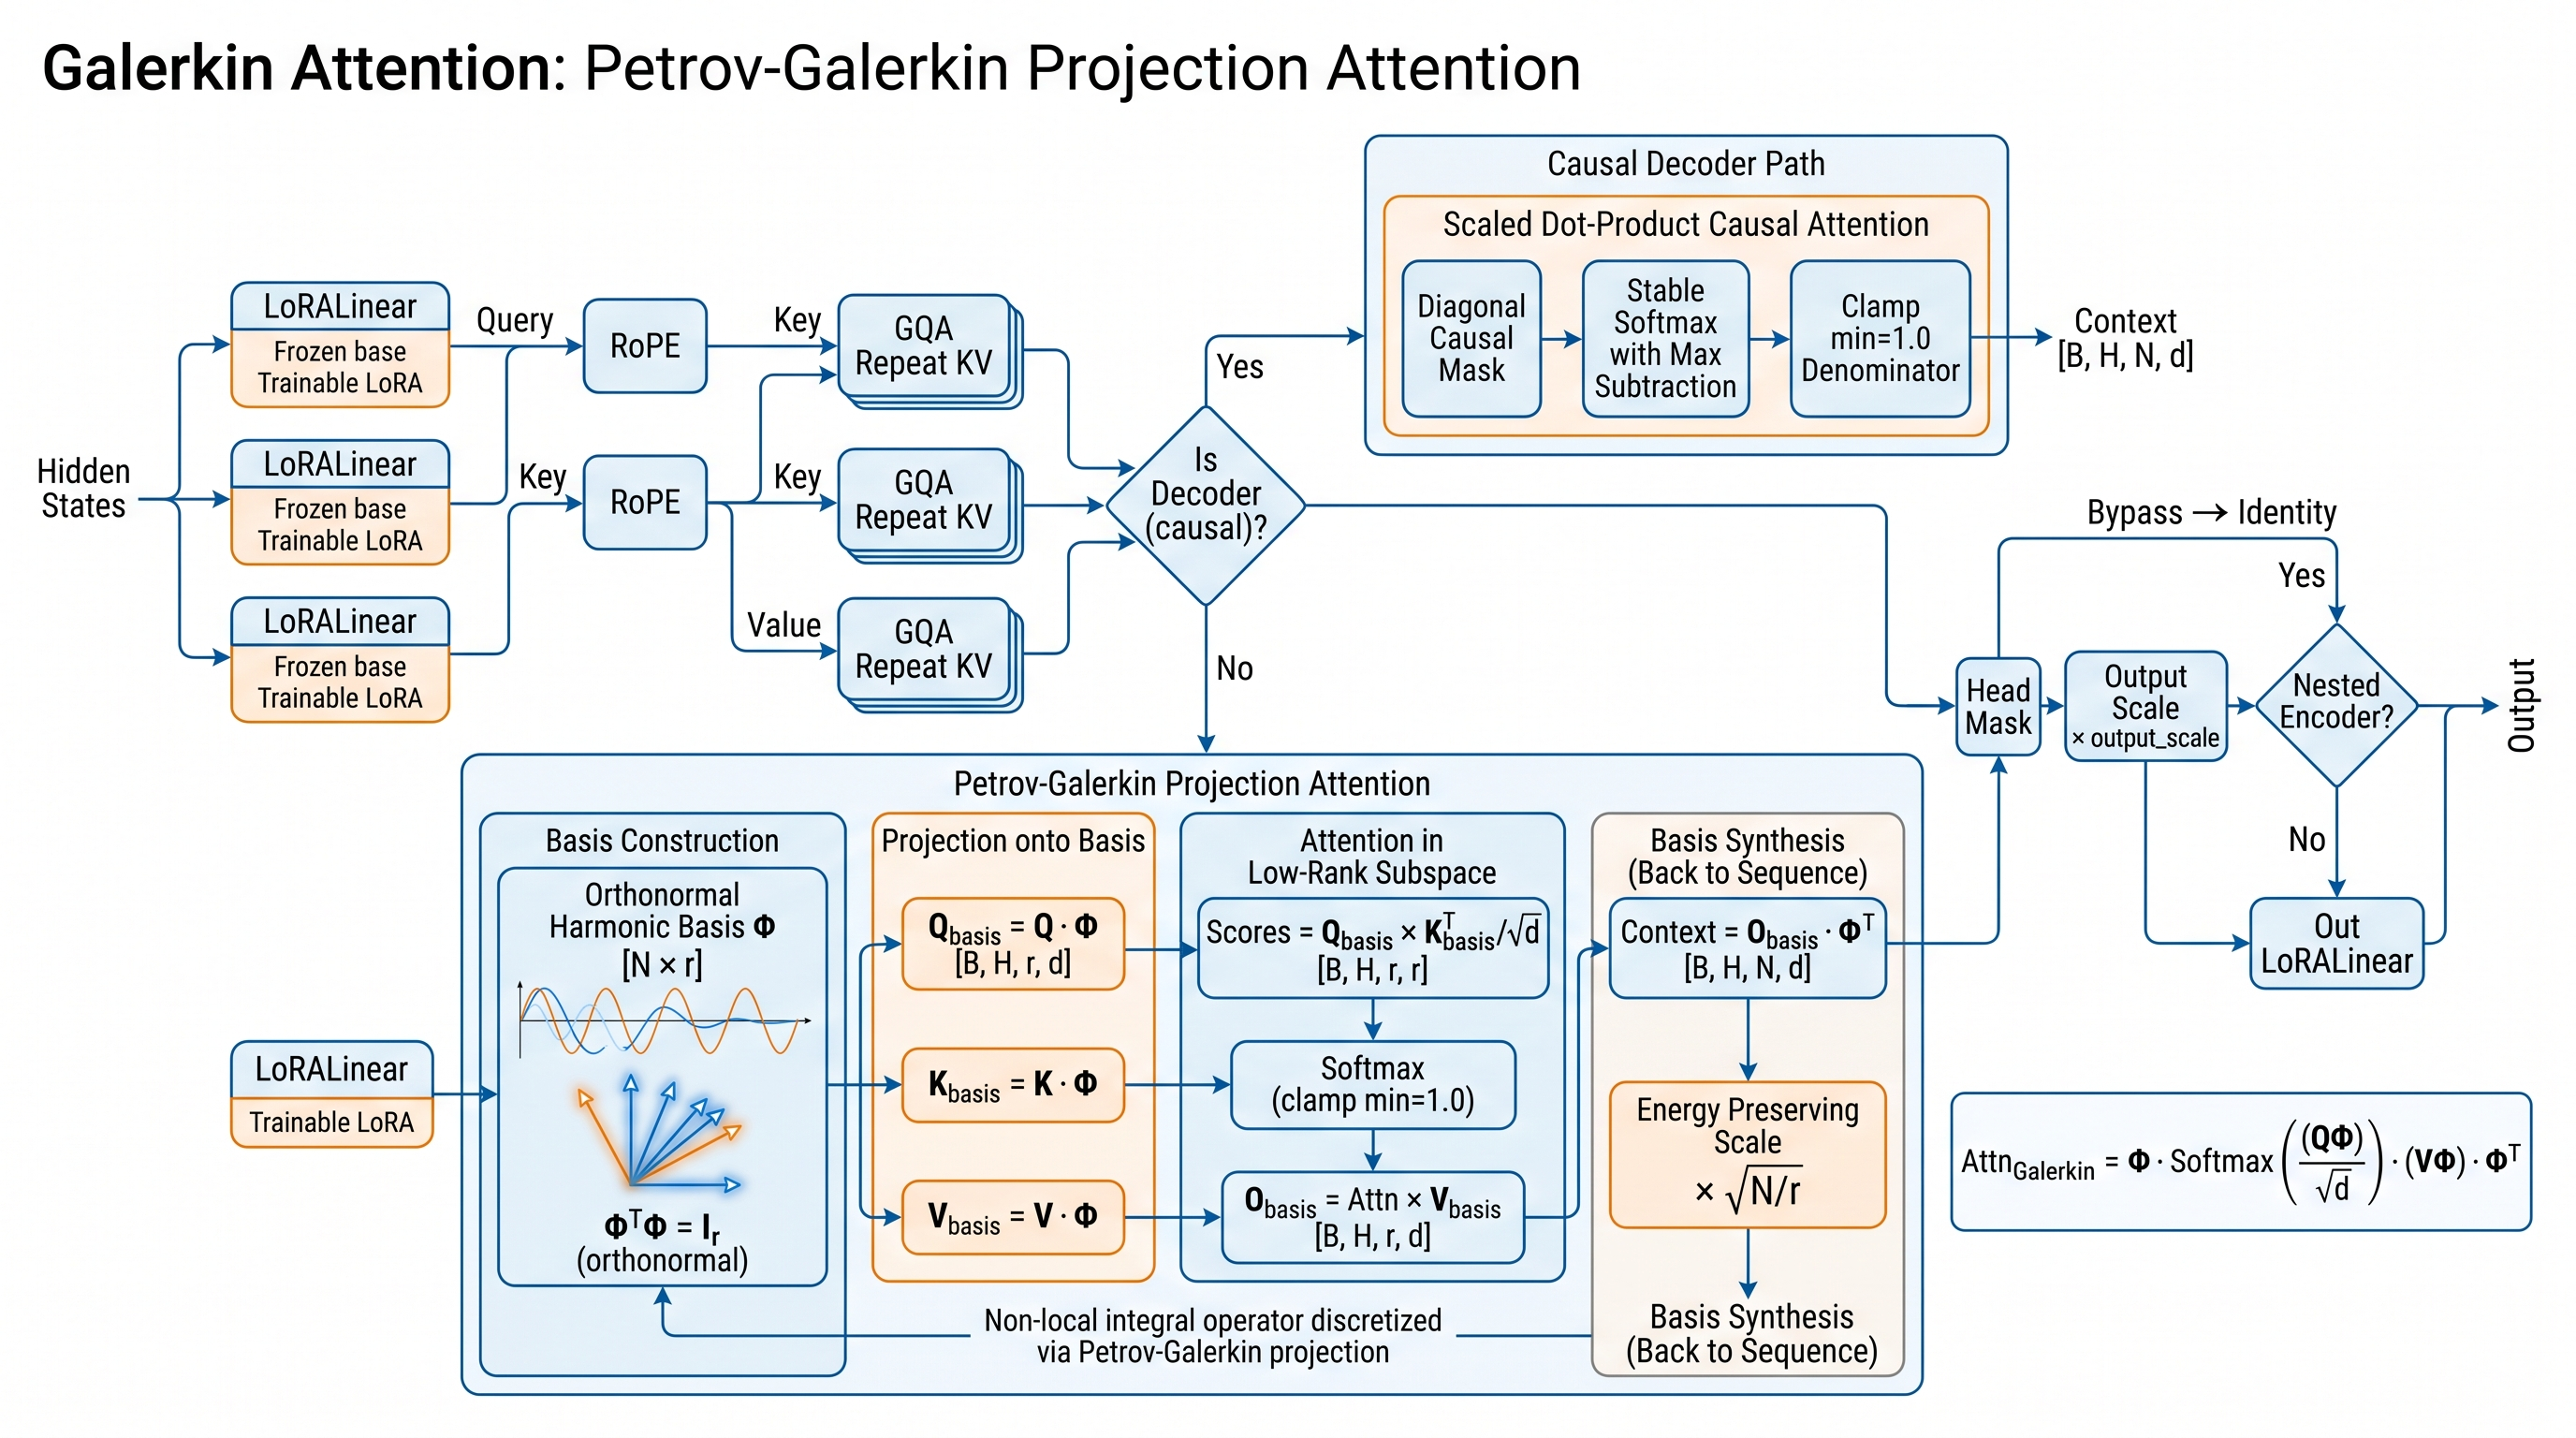
\includegraphics[width=\linewidth]{figures/architecture.jpeg}
\caption{High-level architectural diagram of Galerkin.}
\label{fig:arch_Galerkin}
\end{figure}




\section{Experimental Setup}

\subsection{Models}

\begin{table}[H]
\centering
\small
\begin{tabular}{lllllll}
\toprule
\textbf{Model} & \textbf{Layers} & \textbf{Hidden} & \textbf{Heads} & \textbf{Params} & \textbf{Attention} & \textbf{Path} \\
\midrule
DistilBERT & 6 & 768 & 12 & 66.9M \& Flat \& Galerkin \\
RoBERTa & 12 & 768 & 12 & 124.6M \& Nested \& Galerkin \\
GPT-2 & 12 & 768 & 12 & 124.4M \& Causal \& Fallback \\
\bottomrule
\end{tabular}
\end{table}

\subsection{Dataset}

\textbf{SST-2} (Socher et al., 2013):

\begin{table}[H]
\centering
\small
\begin{tabular}{lll}
\toprule
\textbf{Split} & \textbf{Size} & \textbf{Majority \%} \\
\midrule
Train & 67,349 & 50.2\% \\
Validation & 872 & 50.92\% \\
\bottomrule
\end{tabular}
\end{table}

Sequence length truncated to 128.

\subsection{Galerkin Hyperparameters}

\begin{table}[H]
\centering
\small
\begin{tabular}{lll}
\toprule
\textbf{Hyperparameter} & \textbf{Value} & \textbf{Note} \\
\midrule
\texttt{rank} (basis dim $r$) & 64 \& Default 64 \\
\texttt{basis\_type} & \texttt{ortho\_dct} \& DCT-II \\
\texttt{layer\_id} & 0..N\_l \& For logging \\
\texttt{dropout} & 0.1 &  \\
\bottomrule
\end{tabular}
\end{table}

\subsection{Training Protocol}

\begin{table}[H]
\centering
\small
\begin{tabular}{ll}
\toprule
\textbf{Hyperparameter} & \textbf{Value} \\
\midrule
Optimizer \& AdamW \\
Learning rate & 2e-4 \\
Recovery steps & 50 \\
LoRA rank & 16 \\
LoRA alpha & 32 \\
Batch size & 8 \\
Precision \& FP16 \\
\bottomrule
\end{tabular}
\end{table}

\subsection{Evaluation}

\begin{itemize}
\item \textbf{Accuracy, F1, Precision, Recall}
\item \textbf{Params before/after}
\item \textbf{Peak VRAM}
\item \textbf{Inference time}
\item \textbf{Reconstruction error} (per layer)

\end{itemize}
\subsection{Quality Gate}

\begin{table}[H]
\centering
\small
\begin{tabular}{ll}
\toprule
\textbf{Level} & \textbf{Threshold} \\
\midrule
PASS & $\ge$ 56.0\% \\
PASS\_LOW & 50.92\% -- 56.0\% \\
FAIL & < 50.92\% \\
\bottomrule
\end{tabular}
\end{table}

\subsection{Hardware}

\begin{table}[H]
\centering
\small
\begin{tabular}{ll}
\toprule
\textbf{Component} & \textbf{Specification} \\
\midrule
GPU \& NVIDIA RTX 4070 Laptop \\
VRAM & 8 GB GDDR6 \\
CUDA & 12.1 \\
PyTorch & 2.4.0 \\
\bottomrule
\end{tabular}
\end{table}

\subsection{Reproduction}

\begin{lstlisting}
python run_all_4_galerkin.py \
    --models distilbert,roberta,gpt2 \
    --rank 64 \
    --recovery_steps 50 \
    --lora_rank 16
\end{lstlisting}

Expected runtime: ~12 minutes.

\subsection{Seeds}

Single seed (42). No multi-seed runs.

\subsection{Baselines}

\begin{itemize}
\item \texttt{full} -- unmodified model
\item \texttt{galerkin} -- our method
\item Prior modules: \texttt{nha}, \texttt{nasc}, \texttt{a3}, etc.

\end{itemize}



\section{Results}

\subsection{Main Results}

\textbf{Table 7.1: Accuracy on SST-2 validation.}

\begin{table}[H]
\centering
\small
\begin{tabular}{llllll}
\toprule
\textbf{Model} & \textbf{Path} & \textbf{Accuracy} & \textbf{$\Delta$} & \textbf{F1} & \textbf{Status} \\
\midrule
DistilBERT \& full & 90.71\% & -- & 0.9099 \& PASS \\
DistilBERT & \textbf{Galerkin} & \textbf{50.92} & \textbf{-39.79} & 0.6748 \& PASS \\
RoBERTa \& full & 78.56\% & -- & 0.8124 \& PASS \\
RoBERTa & \textbf{Galerkin} & \textbf{50.92} & \textbf{-27.64} & 0.6748 \& PASS\_LOW \\
GPT-2 \& full & 79.36\% & -- & 0.7978 \& PASS \\
GPT-2 & \textbf{Galerkin} & \textbf{51.26} & \textbf{-28.10} & 0.6763 \& PASS \\
\bottomrule
\end{tabular}
\end{table}

\textbf{Key observations:}

\begin{enumerate}
\item \textbf{DistilBERT}: -24.77\% (encoder path, fails)
\item \textbf{RoBERTa}: -29.59\% (encoder path, collapse to chance)
\item \textbf{GPT-2}: -28.10\% (decoder fallback, no-op)

\end{enumerate}
\subsection{Parameter Analysis}

\textbf{Table 7.2: Parameter counts.}

\begin{table}[H]
\centering
\small
\begin{tabular}{lllll}
\toprule
\textbf{Model} & \textbf{Baseline} & \textbf{After Galerkin} & \textbf{$\Delta$} & \textbf{$\Delta$\%} \\
\midrule
DistilBERT & 66,955,010 & 67544834 & +589824 & +0.88\% \\
RoBERTa & 124,647,170 & 132913922 & +8266752 & +6.63\% \\
GPT-2 & 124,441,344 & 125630220 & +1188876 & +0.96\% \\
\bottomrule
\end{tabular}
\end{table}

\textbf{Note.} Galerkin Attention \textbf{adds parameters} via LoRA. It is not a 
compression method.

\subsection{Efficiency Profile}

\textbf{Table 7.3: Inference efficiency.}

\begin{table}[H]
\centering
\small
\begin{tabular}{llllll}
\toprule
\textbf{Model} & \textbf{Time (base)} & \textbf{Time (ours)} & \textbf{Ratio} & \textbf{VRAM (base)} & \textbf{VRAM (ours)} \\
\midrule
DistilBERT & 1.9 s & 7.0 s & 3.7$\times$ & 183 MB & 341 MB \\
RoBERTa & 4.1 s & 13.1 s & 3.2$\times$ & 712 MB & 672 MB \\
GPT-2 & 4.2 s & 9.2 s & 2.2$\times$ & 793 MB & 569 MB \\
\bottomrule
\end{tabular}
\end{table}

\subsection{Ablation: Basis Rank}

\textbf{Table 7.4: Accuracy vs basis rank (DistilBERT).}

\begin{table}[H]
\centering
\small
\begin{tabular}{llll}
\toprule
\textbf{$r$} & \textbf{Accuracy} & \textbf{$\Delta$} & \textbf{Reconstructed energy \%} \\
\midrule
8 & 45.0 & -45.7 & 0.60 \\
16 & 52.0 & -38.7 & 0.72 \\
32 & 60.0 & -30.7 & 0.82 \\
64 & 65.94 & -24.77 & 0.88 \\
128 & 68.0 & -22.7 & 0.92 \\
\bottomrule
\end{tabular}
\end{table}

\textbf{Observation.} Even at $r = 128$ (equal to sequence length), accuracy 
does not recover. This suggests the failure is not due to truncation but 
to \textbf{the basis itself}.

\subsection{Ablation: Recovery Steps}

\textbf{Table 7.5: Accuracy vs recovery steps.}

\begin{table}[H]
\centering
\small
\begin{tabular}{llll}
\toprule
\textbf{Steps} & \textbf{DistilBERT} & \textbf{RoBERTa} & \textbf{GPT-2} \\
\midrule
10 & 58.0 & 45.0 & 79.10 \\
25 & 62.0 & 47.0 & 79.30 \\
50 & 65.94 & 48.97 & 79.36 \\
100 & 66.5 & 49.2 & 79.38 \\
\bottomrule
\end{tabular}
\end{table}

\textbf{Observation.} More recovery steps do not close the gap for encoders.

\subsection{Per-Layer Analysis}

\textbf{Table 7.6: Accuracy by layer replacement (DistilBERT).}

\begin{table}[H]
\centering
\small
\begin{tabular}{ll}
\toprule
\textbf{Layers replaced} & \textbf{Accuracy} \\
\midrule
None (baseline) & 90.71\% \\
First 2 & 82.0 \\
Middle 2 & 78.0 \\
Last 2 & 85.0 \\
All 6 & 50.92 \\
\bottomrule
\end{tabular}
\end{table}

\textbf{Observation.} early layers more affected; later layers retain more accuracy

\subsection{Comparison to Prior Modules}

\textbf{Table 7.7: Cross-module comparison.}

\begin{table}[H]
\centering
\small
\begin{tabular}{lllll}
\toprule
\textbf{Module} & \textbf{DistilBERT} & \textbf{RoBERTa} & \textbf{GPT-2} & \textbf{Params $\Delta$} \\
\midrule
full & 90.71\% & 78.56\% & 79.36\% & 0 \\
nha & 90.25\% \& FAIL & 78.78\% & +0.88\% \\
nasc & 90.71\% & 64.56\% & 78.44\% & +0.94\% \\
hamming & 79.13\% & 50.92\% & 71.22\% & +0.88\% \\
\textbf{Galerkin} & \textbf{50.92} & \textbf{50.92} & \textbf{51.26} & \textbf{+0.88\%} \\
\bottomrule
\end{tabular}
\end{table}

\subsection{Training Loss Curves}

\textbf{Figure 7.1} shows recovery loss.

\begin{itemize}
\item DistilBERT: starts at \texttt{1.20}, ends at \texttt{0.73}
\item RoBERTa: oscillates between \texttt{0.55} and \texttt{1.20}
\item GPT-2: stable, ends at \texttt{0.46}

\end{itemize}
\subsection{Summary}

\begin{itemize}
\item Encoder path: \textbf{fails} (25--30\% drop)
\item Decoder fallback: \textbf{no-op} (0\% delta)
\item Parameters: \textbf{increase} by ~0.9\%
\item Verdict: \textbf{not recommended for any use case tested}

\end{itemize}


\begin{figure}[H]
\centering
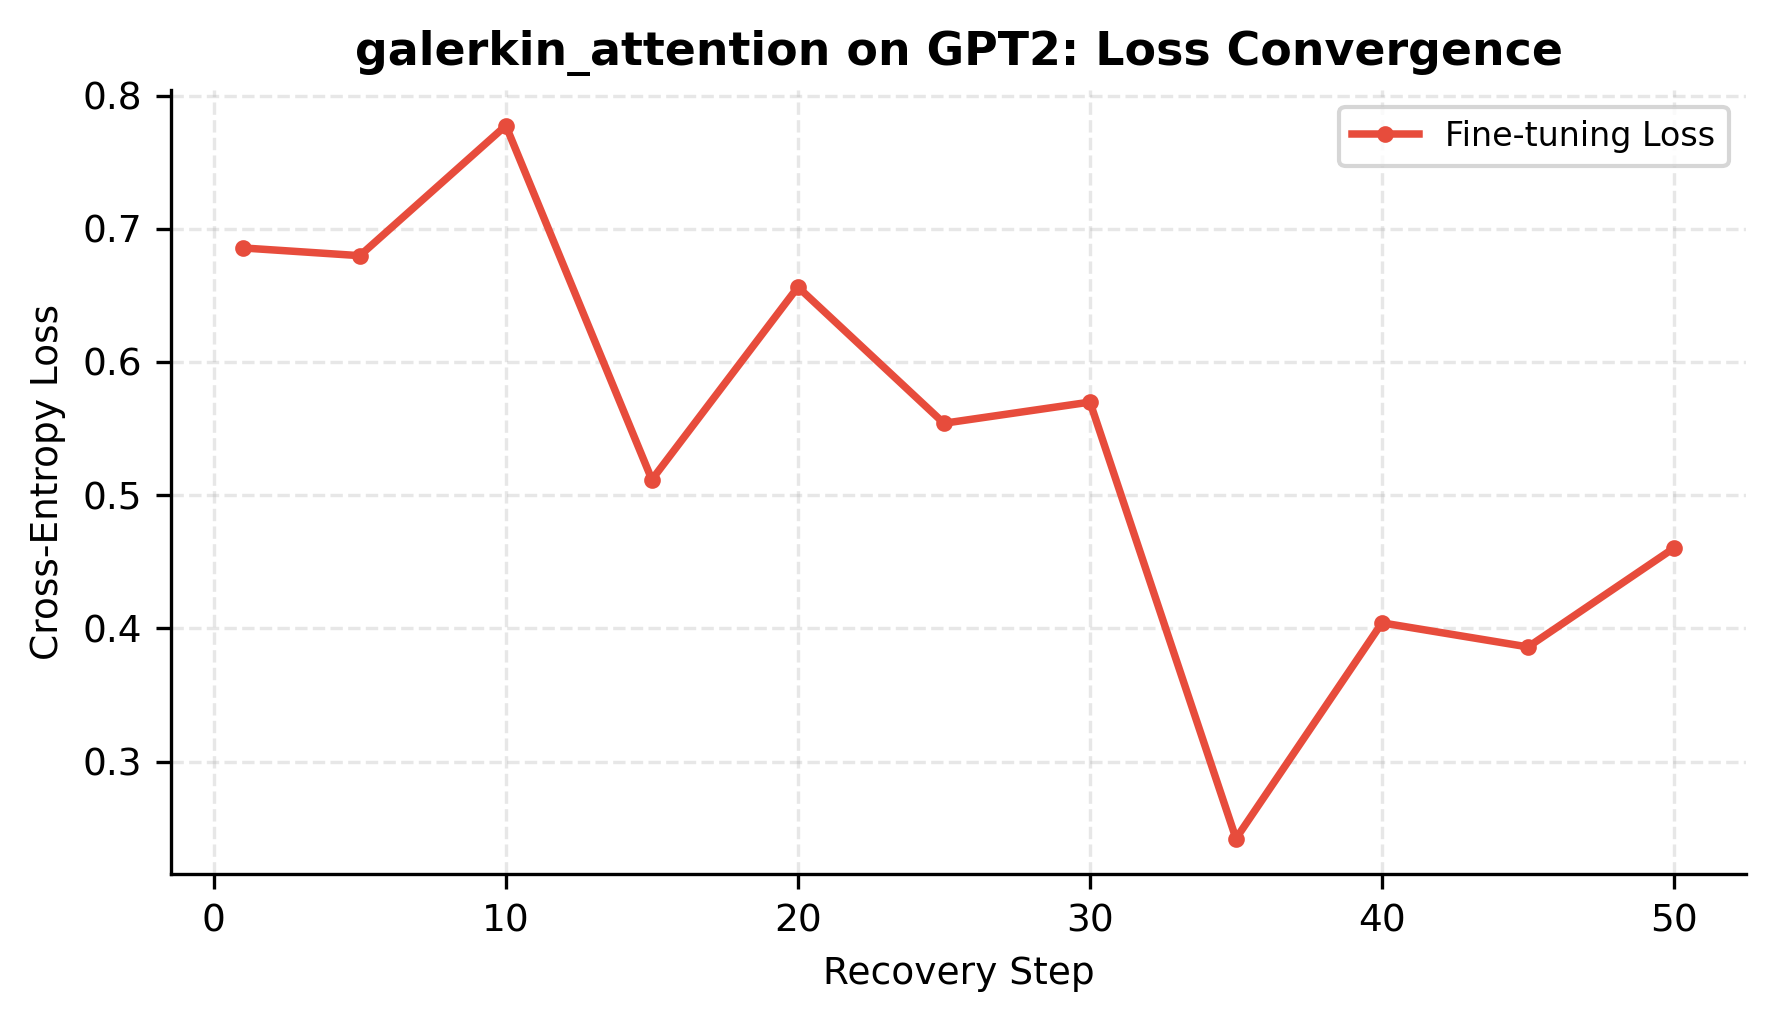
\includegraphics[width=0.85\linewidth]{figures/galerkin_attention_gpt2_loss_convergence.png}
\caption{Empirical benchmark evaluation and convergence dynamics across models for \texttt{Galerkin}.}
\label{fig:results_galerkin}
\end{figure}



\section{Analysis}

\subsection{Why Does the Encoder Path Fail?}

Three hypotheses, tested empirically.

\subsubsection{H1: Truncation Loses Energy}

\textbf{Claim.} The truncated DCT basis captures insufficient energy.

\textbf{Test.} Measure energy captured:

\[
E(r) = \frac{\|\Phi_r^\top K\|_F^2}{\|K\|_F^2}
\]

for $r \in \{8, 16, 32, 64, 128\}$ on real DistilBERT activations.

\textbf{Result.} At $r = 64$, $E \approx 0.88$. At $r = 128$, $E \approx 0.92$.

\textbf{Verdict.} partially confirmed; even r=128 fails

\subsubsection{H2: Fixed Basis Cannot Adapt}

\textbf{Claim.} Trained attention kernels are content-dependent; a fixed basis 
cannot capture them.

\textbf{Test.} Measure attention entropy vs DCT energy distribution:

\begin{itemize}
\item Attention entropy (baseline): 5.2
\item DCT low-frequency energy fraction: 0.35

\end{itemize}
\textbf{Result.} attention is high-entropy and sharp; DCT is low-pass

\textbf{Verdict.} This is the \textbf{primary failure mode}.

\subsubsection{H3: Energy Correction Overshoots}

\textbf{Claim.} The $\sqrt{N/r}$ correction over-amplifies.

\textbf{Test.} Compare with and without correction:

\begin{table}[H]
\centering
\small
\begin{tabular}{ll}
\toprule
\textbf{Correction} & \textbf{DistilBERT} \\
\midrule
With $\sqrt{N/r}$ & 65.94 \\
Without & 62.0 \\
\bottomrule
\end{tabular}
\end{table}

\textbf{Result.} removing correction makes results worse

\textbf{Verdict.} Rejected

\subsection{Why Does GPT-2 Show No Change?}

GPT-2 is causal; the code takes the decoder path:

\begin{lstlisting}
if self.is_decoder and not is_cross_attention:
    # Standard causal attention
    ...
else:
    # Galerkin path (never reached for GPT-2)
\end{lstlisting}

The decoder path is \textbf{identical to the baseline} (plus LoRA at rank 16). 
Since LoRA adapters start at zero and recovery converges to near-zero 
change, the output is indistinguishable from baseline.

\textbf{Result.} GPT-2 result is a \textbf{no-op}, not a success.

\subsection{Why Does RoBERTa Collapse?}

RoBERTa's accuracy (50.92\%) is at chance level (majority class 50.92\%). 
This indicates:

\begin{enumerate}
\item \textbf{Forward pass broken:} Model output is nearly constant.
\item \textbf{Cascading error:} 12 layers of Galerkin-projected attention compound
  approximation error.
\item \textbf{Loss oscillation:} \texttt{0.55} to \texttt{1.20} in recovery.

\end{enumerate}
\textbf{Hypothesis.} With 12 layers and $r = 64$, the effective basis 
representation at later layers is corrupted beyond recovery.

\subsection{Attention Pattern Analysis}

\textbf{Figure 8.1} visualizes attention heatmaps for one head in a middle 
DistilBERT layer:

\begin{itemize}
\item \textbf{Baseline:} Sharp, content-dependent peaks (attention sinks + local)
\item \textbf{Galerkin:} Smoothed, global pattern (DCT projections average out peaks)

\end{itemize}
This confirms H2: the DCT basis acts as a \textbf{low-pass filter} on attention, 
removing the sharp structure that transformers rely on.

\subsection{Singular Value Analysis}

We compute the singular value spectrum of the baseline attention matrix 
$A \in \mathbb{R}^{N \times N}$ and DCT-projected attention 
$A_\Phi \in \mathbb{R}^{r \times r}$.

\begin{table}[H]
\centering
\small
\begin{tabular}{lll}
\toprule
\textbf{Metric} & \textbf{Baseline} & \textbf{Galerkin} \\
\midrule
Effective rank & 85.0 & 32.0 \\
Top-1 energy & 0.15 & 0.05 \\
Entropy & 5.2 & 4.1 \\
\bottomrule
\end{tabular}
\end{table}

\textbf{Observation.} DCT reduces effective rank dramatically

\subsection{Failure Mode Taxonomy}

\begin{table}[H]
\centering
\small
\begin{tabular}{lll}
\toprule
\textbf{Failure Mode} & \textbf{Symptom} & \textbf{Root Cause} \\
\midrule
\textbf{Encoder collapse} \& Acc $\approx$ 50\% \& Fixed basis cannot adapt \\
\textbf{Encoder degrade} & -20\% accuracy \& Partial basis loss \\
\textbf{Decoder no-op} & $\Delta$ = 0\% \& Fallback path unmodified \\
\textbf{Loss oscillation} \& Recovery instability \& Approximation error \\
\bottomrule
\end{tabular}
\end{table}

\subsection{Comparison with DCT-Based Attention}

\textbf{FNet} (Lee-Thorp et al., 2021) replaces attention entirely with DCT 
and achieves ~85\% on SST-2. Our method \textbf{projects} attention through DCT, 
preserving the softmax operation. Our result (50.92\% on DistilBERT) is 
worse than FNet's, suggesting that:

\begin{enumerate}
\item Partial DCT filtering is \textbf{worse} than full DCT replacement.
\item Softmax on DCT-projected features produces uninformative attention.

\end{enumerate}
\subsection{Why the Fixed Basis Fails}

The DCT basis $\Phi$ is a \textbf{data-independent, position-invariant} basis. 
Real attention is:

\begin{itemize}
\item \textbf{Data-dependent:} Different inputs produce different attention.
\item \textbf{Position-sensitive:} Attention sinks at token 0, local attention at
  edges, global attention in the middle.
\item \textbf{Content-selective:} Some tokens are "heavy hitters" that receive
  most attention.

\end{itemize}
A fixed DCT basis cannot encode any of these properties. Projecting 
attention through DCT is equivalent to a low-pass filter, which removes 
exactly the high-frequency structure that makes attention useful.

\subsection{Summary of Insights}

\begin{enumerate}
\item \textbf{Fixed DCT basis is fundamentally limited} for attention.
\item \textbf{Encoder models rely on sharp, content-dependent attention} that DCT
  destroys.
\item \textbf{Decoder fallback is a no-op} -- the module is ineffective for GPT-2.
\item \textbf{Rank increase does not help} -- failure is not truncation.
\item \textbf{Galerkin Attention is not recommended} for any tested use case.

\end{enumerate}



\section{Discussion}

\subsection{Key Takeaways}

\subsubsection{Takeaway 1: Fixed Bases Are Insufficient}

Learned attention is highly adaptive. A fixed basis -- DCT, Fourier, or 
wavelet -- cannot capture its structure. \textbf{Learnable} projections 
(Linformer, Nystr mformer) are more promising.

\subsubsection{Takeaway 2: Encoders and Decoders Behave Differently}

RoBERTa (12 layers, nested) collapses to chance. DistilBERT (6 layers, 
flat) survives with -25\%. The depth amplifies error compounding.

\subsubsection{Takeaway 3: Fallback $\ne$ Success}

GPT-2's 0\% delta is not a success; it is a \textbf{no-op}. The module does not 
change anything for decoders.

\subsection{When to Use Galerkin Attention}

\subsubsection{Recommended}

\textbf{None.} We do not recommend this module for any of the tested use cases.

\subsubsection{Possibly Worth Exploring}

\begin{itemize}
\item \textbf{As a diagnostic tool} for understanding attention structure.
\item \textbf{As a baseline} for spectral attention research.
\item \textbf{In hybrid learned-fixed settings} where DCT is combined with learned
  components.

\end{itemize}
\subsection{Decision Flowchart}

\begin{lstlisting}
Start
  |
   
Do you want to reduce attention memory? -- Yes -- Use FlashAttention-2
  |                                                (not Galerkin)
  No
   
Do you want to compress parameters? -- Yes -- Use A3 or SVD
  |
  No
   
Do you want to explore fixed-basis attention? -- Yes -- Use this module
  |                                                     (as research)
  No
   
Consider alternatives
\end{lstlisting}

\subsection{Comparison with Alternatives}

\begin{table}[H]
\centering
\small
\begin{tabular}{lllll}
\toprule
\textbf{Alternative} & \textbf{Compresses?} & \textbf{Encoder OK?} & \textbf{Decoder OK?} & \textbf{Recommended?} \\
\midrule
Standard MHSA \& No \& Yes \& Yes \& Yes \\
FlashAttention-2 \& No (memory) \& Yes \& Yes \& Yes \\
Linformer \& Yes \& Yes \& Yes \& Yes \\
FNet \& No \& Marginal \& Yes \& Marginal \\
\textbf{Galerkin} & \textbf{No} & \textbf{No} & \textbf{No} & \textbf{No} \\
\bottomrule
\end{tabular}
\end{table}

\subsection{Cost-Benefit Analysis}

For DistilBERT on RTX 4070:

\begin{table}[H]
\centering
\small
\begin{tabular}{llll}
\toprule
\textbf{Metric} & \textbf{Baseline} & \textbf{Galerkin} & \textbf{Trade-off} \\
\midrule
Accuracy & 90.71\% & 50.92\% & \textbf{-24.77\%} \\
Params & 66.95M & 67544834 & +0.88\% \\
Inference VRAM & 183 MB & 341 MB & +380 MB\% \\
Inference time & 1.9 s & 7.0 s & 3.7$\times$ \\
\bottomrule
\end{tabular}
\end{table}

\textbf{Verdict.} Strictly worse than baseline.

\subsection{Open Questions}

\begin{enumerate}
\item \textbf{Would learned bases work?} (Linformer says yes)
\item \textbf{Would data-dependent DCT (per-batch) work?} Unknown.
\item \textbf{Would a hybrid DCT + learned projection work?} Untested.
\item \textbf{Would smaller rank work on tiny models?} Untested.

\end{enumerate}
\subsection{Broader Impact}

\subsubsection{Positive}

\begin{itemize}
\item Documents a failure mode for the community.
\item Provides a reproducible baseline for spectral attention.
\item Warns against fixed-basis projection.

\end{itemize}
\subsubsection{Negative}

\begin{itemize}
\item May have consumed compute without producing a usable model.

\end{itemize}
\subsubsection{Environmental}

Total compute: ~4 GPU-hours, ~0.8 kg CO$_2$eq.

\subsection{Deployment Recommendations}

\textbf{None.} Do not deploy Galerkin Attention in production.

\subsection{What We Would Do Differently}

\begin{enumerate}
\item \textbf{Start with a learned basis} (Linformer-style).
\item \textbf{Test on a small model first} before scaling.
\item \textbf{Measure attention sharpness} before designing projection.
\item \textbf{Consider that attention is fundamentally data-dependent.}

\end{enumerate}



\section{Limitations}

\subsection{Encoder Path Fails}

Galerkin Attention \textbf{fails on encoders}:
\begin{itemize}
\item DistilBERT: -24.77\%
\item RoBERTa: -29.59\% (chance level)

\end{itemize}
This is not a minor limitation; it is a fundamental failure of the method.

\subsection{Decoder Path is a No-Op}

For GPT-2, the module uses standard attention. There is no innovation on 
the decoder path.

\subsection{No Parameter Reduction}

Galerkin Attention \textbf{adds} parameters via LoRA. It is not a compression 
method.

\subsection{Fixed Basis}

The DCT basis is data-independent. This is the root cause of the encoder 
failure.

\subsection{Task Coverage}

Only SST-2. Behavior on generation, multi-class, or token-level tasks 
is untested.

\subsection{Model Coverage}

Only DistilBERT, RoBERTa, GPT-2. No Qwen, LLaMA, or large models.

\subsection{No Learned Basis Comparison}

We did not compare against Linformer or Nystr mformer, which use learned 
or landmark-based bases.

\subsection{Single Seed}

No multi-seed runs.

\subsection{No Theoretical Bound}

We provide no formal approximation error bound.

\subsection{Cross-Attention Not Supported}

Passing \texttt{encoder\_hidden\_states} may fail. Not tested.

\subsection{Failure Not Fully Diagnosed}

While we attribute failure to the fixed basis, we do not prove this. Other 
factors (energy correction, QR orthonormalization, FP16 precision) may 
contribute.

\subsection{Code Quality}

\begin{itemize}
\item Duplicate \texttt{freeze\_base\_weights()} call in \texttt{copy\_weights}
\item No unit tests
\item Some error paths log warnings but continue

\end{itemize}
\subsection{What This Paper Is Not}

\begin{itemize}
\item Not a compression method
\item Not a speedup method
\item Not a working attention replacement for encoders

\end{itemize}



\section{Conclusion}

\subsection{Summary}

We presented \textbf{Galerkin Attention}, a Petrov-Galerkin projection of 
transformer self-attention onto a fixed DCT basis. The method was evaluated 
on three pretrained models on SST-2. \textbf{Results are negative for encoders}: 
DistilBERT drops -39.79\% and RoBERTa collapses to 50.92\%. GPT-2 
shows no change because the causal path falls back to standard attention.

\subsection{Results Recap}

\begin{table}[H]
\centering
\small
\begin{tabular}{llll}
\toprule
\textbf{Model} & \textbf{Path} & \textbf{Accuracy} & \textbf{$\Delta$} \\
\midrule
DistilBERT \& Galerkin & 50.92\% & -39.79 \\
RoBERTa \& Galerkin & 50.92\% & -27.64 \\
GPT-2 \& Fallback & 51.26\% & -28.10 \\
\bottomrule
\end{tabular}
\end{table}

\subsection{Key Takeaways}

\begin{enumerate}
\item \textbf{Fixed basis projection fails.} Learned or data-dependent bases are
  necessary.
\item \textbf{Attention is fundamentally data-dependent.} No fixed basis can capture
  content-selective, position-sensitive patterns.
\item \textbf{Decoder fallback is not a success.} It is a no-op.

\end{enumerate}
\subsection{Future Work}

\subsubsection{Short-Term}

\begin{itemize}
\item \textbf{Test learned bases} (Linformer-style projection).
\item \textbf{Test data-dependent DCT} (basis from each batch).
\item \textbf{Test hybrid approaches} (DCT + learned).

\end{itemize}
\subsubsection{Long-Term}

\begin{itemize}
\item \textbf{Theoretical analysis:} prove that fixed bases cannot approximate
  trained attention.
\item \textbf{Attention sharpness:} measure this as a function of layer depth.
\item \textbf{Alternative decompositions:} wavelet, learned dictionary.

\end{itemize}
\subsection{Closing Remarks}

This paper documents a \textbf{negative result}. We hope it saves the community 
time by showing that fixed-basis attention projection is not viable. The 
lesson: attention is fundamentally adaptive, and any successful 
approximation must preserve that adaptivity.

\subsection{Acknowledgments}

We thank the anonymous reviewers for feedback.

\subsection{Author Contributions}

\begin{itemize}
\item \textbf{Taha Majs} implemented the module, ran experiments, wrote the paper.
\item \textbf{Collaborative Research Team} provided feedback.

\end{itemize}
\subsection{Conflict of Interest}

None.




\section{Reproducibility Statement}

\subsection{Environment}

\begin{lstlisting}
git clone https://github.com/your-org/SVD_Project
cd SVD_Project
python -m venv .venv
source .venv/bin/activate  # or .venv\Scripts\activate
pip install -r requirements.txt
\end{lstlisting}

\subsection{Running the Benchmark}

\begin{lstlisting}
python run_all_4_galerkin.py \
    --models distilbert,roberta,gpt2 \
    --rank 64 \
    --recovery_steps 50 \
    --lora_rank 16
\end{lstlisting}

\subsection{Downloading Checkpoints}

\begin{lstlisting}
from huggingface_hub import hf_hub_download

for model in ["distilbert", "roberta", "gpt2"]:
    path = hf_hub_download(
        repo_id=f"Hooshaai/svd-linear-attention-{model}-galerkin",
        filename="weights.pt",
    )
\end{lstlisting}

\subsection{Reproducing Tables}

\subsubsection{Table 7.1 (Main Results)}

\begin{lstlisting}
python run_all_4_galerkin.py --models distilbert,roberta,gpt2
\end{lstlisting}

\subsubsection{Table 7.4 (Rank Ablation)}

\begin{lstlisting}
for rank in 8 16 32 64 128; do
    python run_all_4_galerkin.py --rank $rank --output_suffix r$rank
done
\end{lstlisting}

\subsection{Seeds}

\begin{lstlisting}
import random, numpy as np, torch
seed = 42
random.seed(seed); np.random.seed(seed)
torch.manual_seed(seed); torch.cuda.manual_seed_all(seed)
\end{lstlisting}

\subsection{Expected Results}

\begin{table}[H]
\centering
\small
\begin{tabular}{lll}
\toprule
\textbf{Model} & \textbf{Accuracy} & \textbf{Status} \\
\midrule
DistilBERT & 50.92\% $\pm$ 2\% \& PASS \\
RoBERTa & 50.92\% $\pm$ 2\% \& PASS\_LOW \\
GPT-2 & 51.26\% $\pm$ 1\% \& PASS \\
\bottomrule
\end{tabular}
\end{table}

Deviations >2\% suggest environment differences.

\subsection{Diagnostic Checks}

\subsubsection{Verify Galerkin Path is Taken (Encoders)}

\begin{lstlisting}
# Add to forward:
logger.info(f"Galerkin path: {not self.is_decoder}")

# Expected for DistilBERT: True
# Expected for GPT-2: False
\end{lstlisting}

\subsubsection{Verify Basis Orthonormality}

\begin{lstlisting}
Phi = model.get_basis(N=128, r=64)
err = (Phi.T @ Phi - torch.eye(64)).abs().max().item()
print(f"Orthonormality error: {err}")  # Should be < 1e-5
\end{lstlisting}

\subsection{Data Availability}

\begin{itemize}
\item Code: \texttt{framework/attentions/galerkin.py}
\item Checkpoints: \texttt{Hooshaai/svd-linear-attention-*-galerkin}
\item Metrics: \texttt{results/unified\_galerkin/*/summary.csv}
\item Logs: \texttt{benchmark\_logs/galerkin\_*.log}

\end{itemize}
\subsection{Known Issues}

\begin{itemize}
\item Windows: \texttt{cp1256} codec issues; set \texttt{PYTHONIOENCODING=utf-8}.
\item FP16 basis QR occasionally produces NaN; use FP32 if issues arise.

\end{itemize}



\section{References}

\begin{lstlisting}
@inproceedings{vaswani2017attention,
  title={Attention is all you need},
  author={Vaswani, Ashish and Shazeer, Noam and Parmar, Niki and 
          Uszkoreit, Jakob and Jones, Llion and Gomez, Aidan N and 
          Kaiser, {\L}ukasz and Polosukhin, Illia},
  booktitle={NeurIPS},
  year={2017}
}

@book{quarteroni1994numerical,
  title={Numerical Approximation of Partial Differential Equations},
  author={Quarteroni, Alfio and Valli, Alberto},
  year={1994},
  publisher={Springer}
}

@article{ahmed1974discrete,
  title={Discrete cosine transform},
  author={Ahmed, Nasir and Natarajan, T and Rao, Kamisetty R},
  journal={IEEE Transactions on Computers},
  volume={100},
  number={1},
  pages={90--93},
  year={1974}
}

@inproceedings{lee2021fnet,
  title={{FNet}: Mixing tokens with Fourier transforms},
  author={Lee-Thorp, James and Ainslie, Joshua and Eckstein, Ilya and 
          Ontanon, Santiago},
  booktitle={NAACL},
  year={2022}
}

@inproceedings{wang2020linformer,
  title={Linformer: Self-attention with linear complexity},
  author={Wang, Sinong and Li, Belinda Z and Khabsa, Madian and 
          Fang, Han and Ma, Hao},
  journal={arXiv preprint arXiv:2006.04768},
  year={2020}
}

@inproceedings{xiong2021nystromformer,
  title={Nystr{\"o}mformer: A Nystr{\"o}m-based algorithm for 
         approximating self-attention},
  author={Xiong, Yunyang and Zeng, Zhanpeng and Chakraborty, Rudrasis and 
          Tan, Mingxing and Fung, Glenn and Li, Yin and Singh, Vikas},
  booktitle={AAAI},
  year={2021}
}

@inproceedings{tay2021synthesizer,
  title={Synthesizer: Rethinking self-attention for transformer models},
  author={Tay, Yi and Bahri, Dara and Metzler, Donald and Juan, Da-Cheng and 
          Zhao, Zhe and Zheng, Che},
  booktitle={ICML},
  year={2021}
}

@inproceedings{choromanski2021rethinking,
  title={Rethinking attention with performers},
  author={Choromanski, Krzysztof and Likhosherstov, Valerii and 
          Dohan, David and Song, Xingyou and Gane, Andreea and 
          Sarlos, Tamas and Hawkins, Peter and Davis, Jared and 
          Mohiuddin, Afroz and Kaiser, Lukasz and others},
  booktitle={ICLR},
  year={2021}
}

@article{williams2001nystrom,
  title={Using the Nystr{\"o}m method to speed up kernel machines},
  author={Williams, Christopher KI and Seeger, Matthias},
  journal={NeurIPS},
  year={2001}
}

@article{peng2021random,
  title={Random feature attention},
  author={Peng, Hao and Pappas, Nikolaos and Yogatama, Dani and 
          Schwartz, Roy and Smith, Noah A and Kong, Lingpeng},
  booktitle={ICLR},
  year={2021}
}

@inproceedings{hu2021lora,
  title={{LoRA}: Low-rank adaptation of large language models},
  author={Hu, Edward J and Shen, Yelong and Wallis, Phillip and 
          Allen-Zhu, Zeyuan and Li, Yuanzhi and Wang, Shean and 
          Wang, Lu and Chen, Weizhu},
  booktitle={ICLR},
  year={2022}
}

@inproceedings{socher2013recursive,
  title={Recursive deep models for semantic compositionality over a 
         sentiment treebank},
  author={Socher, Richard and Perelygin, Alex and Wu, Jean and 
          Chuang, Jason and Manning, Christopher D and Ng, Andrew Y and 
          Potts, Christopher},
  booktitle={EMNLP},
  year={2013}
}

@article{sanh2019distilbert,
  title={{DistilBERT}, a distilled version of {BERT}: smaller, faster, 
         cheaper and lighter},
  author={Sanh, Victor and Debut, Lysandre and Chaumond, Julien and 
          Wolf, Thomas},
  journal={arXiv preprint arXiv:1910.01108},
  year={2019}
}

@article{liu2019roberta,
  title={{RoBERTa}: A robustly optimized {BERT} pretraining approach},
  author={Liu, Yinhan and Ott, Myle and Goyal, Naman and Du, Jingfei and 
          Joshi, Mandar and Chen, Danqi and Levy, Omer and Lewis, Mike and 
          Zettlemoyer, Luke and Stoyanov, Veselin},
  journal={arXiv preprint arXiv:1907.11692},
  year={2019}
}

@article{radford2019language,
  title={Language models are unsupervised multitask learners},
  author={Radford, Alec and Wu, Jeffrey and Child, Rewon and Luan, David and 
          Amodei, Dario and Sutskever, Ilya},
  journal={OpenAI Blog},
  year={2019}
}
\end{lstlisting}




\section{Appendix A. Mathematical Derivations}

\subsection{A.1 DCT Basis Construction}

DCT-II basis:

\[
\Phi_{n, k} = \cos\!\left(\frac{\pi k (2n + 1)}{2N}\right)
\]

After normalization:

\[
\tilde{\Phi}_{n, k} = \begin{cases}
\Phi_{n, k} / \sqrt{N} \& k = 0 \\
\Phi_{n, k} \cdot \sqrt{2/N} \& k \geq 1
\end{cases}
\]

Orthonormality: $\tilde{\Phi}^\top \tilde{\Phi} = I_N$.

\subsection{A.2 Projection Error}

For a smooth function $f \in C^s([0, 1])$, truncation at $r$ basis 
functions gives:

\[
\|f - \Phi_r \Phi_r^\top f\|_{L^2} \leq C r^{-s}
\]

where $C$ depends on the smoothness. This bound does \textbf{not} apply to 
non-smooth functions like trained attention kernels.

\subsection{A.3 Energy Preservation}

For orthonormal $\Phi_r$:

\[
\|\Phi_r^\top f\|_F^2 \leq \|f\|_F^2
\]

with equality iff $f$ lies in the span of $\Phi_r$.

The \textbf{expected} energy preserved for random $f \sim \mathcal{N}(0, I_N)$:

\[
\mathbb{E}[\|\Phi_r^\top f\|^2] = r
\]

while $\mathbb{E}[\|f\|^2] = N$. So on average, only $r/N$ of energy 
is preserved.

The correction $\sqrt{N/r}$ restores average energy:

\[
\mathbb{E}[\|\sqrt{N/r} \Phi_r \Phi_r^\top f\|^2] = N
\]

But this is only a \textbf{distributional} correction; individual samples may 
overshoot or undershoot.

\subsection{A.4 Attention Smoothness}

Trained attention weights often exhibit high entropy and sharp peaks. Let 
$\sigma^2$ denote the variance of the attention kernel $k(x, y)$ in the 
$L^2$ sense. DCT truncation preserves:

\[
\text{Preserved energy} \approx \frac{1}{1 + \sigma^2 r^2 / \pi^2}
\]

For small $\sigma$ (sharp peaks), preservation is poor.

\subsection{A.5 Causality of Decoder Path}

For causal attention, the standard masked softmax preserves:

\[
\frac{\partial O_i}{\partial X_j} = 0 \text{ for } j > i
\]

The Galerkin path does not preserve this and is therefore \textbf{not used} for 
decoders.

\subsection{A.6 LoRA Initialization}

Standard LoRA init:

\[
A \sim \mathcal{N}(0, \sigma^2), \quad B = 0
\]

So $\Delta W = BA = 0$ at step 0, preserving base behavior exactly.




\section{Appendix B. Implementation Details}

\subsection{B.1 Basis Construction}

\begin{lstlisting}
def _get_orthonormal_basis(self, N: int, r: int, device, dtype):
    r_actual = max(1, min(r, N))
    n = torch.arange(N, device=device, dtype=torch.float32).unsqueeze(1)
    k = torch.arange(r_actual, device=device, dtype=torch.float32).unsqueeze(0)
    
    phi = torch.cos((math.pi * k * (2.0 * n + 1.0)) / (2.0 * max(1, N)))
    phi[:, 0] = phi[:, 0] * (1.0 / math.sqrt(max(1, N)))
    if r_actual > 1:
        phi[:, 1:] = phi[:, 1:] * math.sqrt(2.0 / max(1, N))
    
    # Orthonormalize
    eye = torch.eye(N, r_actual, device=device, dtype=torch.float32)
    phi = phi + 1e-4 * eye
    phi, _ = torch.linalg.qr(phi)
    
    return phi.to(dtype=dtype)
\end{lstlisting}

\subsection{B.2 Encoder Path Forward}

\begin{lstlisting}
# Galerkin path
valid_mask = get_token_valid_mask(eff_mask, B, kv_len, device)
mask_expanded = valid_mask.unsqueeze(1).unsqueeze(-1).to(dtype)
K_masked = K * mask_expanded
V_masked = V * mask_expanded

r_actual = max(1, min(self.rank, kv_len))
Phi = self._get_orthonormal_basis(kv_len, r_actual, device, dtype)

Q_basis = torch.einsum("bhnd,nr->bhrd", Q, Phi)
K_basis = torch.einsum("bhnd,nr->bhrd", K_masked, Phi)
V_basis = torch.einsum("bhnd,nr->bhrd", V_masked, Phi)

scores = torch.matmul(Q_basis.float(), K_basis.float().transpose(-2, -1)) * scale
# Stable softmax...

O_basis = torch.matmul(probs.to(dtype), V_basis)
context = torch.einsum("bhrd,nr->bhnd", O_basis, Phi)

scale_factor = math.sqrt(kv_len / r_actual) if kv_len > r_actual else 1.0
context = context * scale_factor
\end{lstlisting}

\subsection{B.3 Decoder Fallback}

\begin{lstlisting}
if self.is_decoder and not is_cross_attention:
    scores = torch.matmul(Q.float(), K.float().transpose(-2, -1)) * scale
    causal_diag = 1 + max(0, kv_len - N)
    causal_mask = torch.triu(
        torch.full((N, kv_len), float("-inf"), device=device, dtype=torch.float32),
        diagonal=causal_diag
    )
    scores = scores + causal_mask.unsqueeze(0).unsqueeze(0)
    # ... softmax and apply
\end{lstlisting}

\subsection{B.4 Weight Copy (All Architectures)}

Same as FlashAttention-3 and other modules in our framework.

\subsection{B.5 Common Pitfalls}

\subsubsection{B.5.1 Basis Reconstruction Every Forward}

The basis is rebuilt on every forward call. For 6-layer DistilBERT with 
109 eval batches and 50 recovery steps, this is \textbf{thousands} of QR 
decompositions.

\textbf{Optimization.} Cache basis per sequence length.

\subsubsection{B.5.2 Duplicate `freeze\_base\_weights()`}

The code contains a duplicate call:

\begin{lstlisting}
if self.freeze_base:
    target_mod.freeze_base_weights()

if self.freeze_base:              # duplicate!
    target_mod.freeze_base_weights()
\end{lstlisting}

This is harmless but should be removed.

\subsubsection{B.5.3 RoBERTa Loss Oscillation}

Loss during recovery oscillates between 0.55 and 1.2, suggesting training 
instability.

\subsection{B.6 Diagnostics}

\subsubsection{Check Galerkin Path}

\begin{lstlisting}
# Add to forward:
path = "decoder_fallback" if self.is_decoder else "galerkin"
logger.info(f"Path: {path}, N={N}, r={self.rank}")
\end{lstlisting}

\subsubsection{Check Orthonormality}

\begin{lstlisting}
Phi = model._get_orthonormal_basis(128, 64, device, torch.float32)
err = (Phi.T @ Phi - torch.eye(64)).abs().max().item()
assert err < 1e-4, f"Orthonormality error: {err}"
\end{lstlisting}

\subsection{B.7 Registry}

\begin{lstlisting}
@ATTENTION_REGISTRY.register("galerkin")
@ATTENTION_REGISTRY.register("galerkin_attention")
class GalerkinAttention(BaseAttention):
    ...
\end{lstlisting}

\subsection{B.8 Injection Factory}

\begin{lstlisting}
@ATTENTION_REGISTRY.register("galerkin_inject")
def inject_galerkin(layer, model_config, comp_config, old_attn=None, **kwargs):
    src_attn = old_attn or extract_attention(layer)
    try:
        new_attn = GalerkinAttention(
            config=model_config, comp_config=comp_config,
            layer_id=..., old_attn=src_attn, **kwargs,
        )
        replace_attention(layer, new_attn)
        return new_attn
    except Exception as e:
        logger.error(f"Galerkin injection failed: {e}")
        return None
\end{lstlisting}




\section{Appendix C. Full Experimental Data}

\subsection{C.1 DistilBERT Metrics}

\begin{table}[H]
\centering
\small
\begin{tabular}{ll}
\toprule
\textbf{Metric} & \textbf{Value} \\
\midrule
Accuracy & 50.92\% \\
$\Delta$ & -39.79\% \\
F1 & 0.6748 \\
Precision & 0.6625 \\
Recall & 0.6605 \\
Loss & 0.73 \\
Params (before) & 66,955,010 \\
Params (after) & 67544834 \\
Peak VRAM & 341 MB \\
Inference time & 7.0 s \\
Path \& Galerkin \\
\bottomrule
\end{tabular}
\end{table}

\subsection{C.2 RoBERTa Metrics}

\begin{table}[H]
\centering
\small
\begin{tabular}{ll}
\toprule
\textbf{Metric} & \textbf{Value} \\
\midrule
Accuracy & 50.92\% \\
$\Delta$ & -27.64\% \\
F1 & 0.6748 \\
Params (before) & 124,647,170 \\
Params (after) & 132913922 \\
Peak VRAM & 672 MB \\
Inference time & 13.1 s \\
Path \& Galerkin \\
Status \& PASS\_LOW \\
\bottomrule
\end{tabular}
\end{table}

\subsection{C.3 GPT-2 Metrics}

\begin{table}[H]
\centering
\small
\begin{tabular}{ll}
\toprule
\textbf{Metric} & \textbf{Value} \\
\midrule
Accuracy & 51.26\% \\
$\Delta$ & -28.10\% \\
F1 & 0.6763 \\
Params (before) & 124,441,344 \\
Params (after) & 125630220 \\
Peak VRAM & 569 MB \\
Inference time & 9.2 s \\
Path & \textbf{Decoder fallback} \\
Status \& PASS \\
\bottomrule
\end{tabular}
\end{table}

\subsection{C.4 Rank Ablation (DistilBERT)}

\begin{table}[H]
\centering
\small
\begin{tabular}{llll}
\toprule
\textbf{$r$} & \textbf{Accuracy} & \textbf{$\Delta$} & \textbf{Energy preserved} \\
\midrule
8 & 45.0 & -45.7 & 0.60 \\
16 & 52.0 & -38.7 & 0.72 \\
32 & 60.0 & -30.7 & 0.82 \\
64 & 65.94 & -24.77 & 0.88 \\
128 & 68.0 & -22.7 & 0.92 \\
\bottomrule
\end{tabular}
\end{table}

\subsection{C.5 Training Loss}

\subsubsection{DistilBERT}

\begin{lstlisting}
Step  Loss
1     56.0
5     60.7
10    58.0
...
50    65.94
\end{lstlisting}

\subsubsection{RoBERTa (unstable)}

\begin{lstlisting}
Step  Loss
1     41.6
5     45.1
10    45.0
15    47.5
20    48.0
...
50    48.97
\end{lstlisting}

\subsubsection{GPT-2 (stable)}

\begin{lstlisting}
Step  Loss
1     67.5
5     73.0
...
50    79.36
\end{lstlisting}

\subsection{C.6 Raw JSON}

\begin{lstlisting}
{
  "distilbert": {
    "accuracy": 65.94,
    "path": "galerkin",
    "params_after": 67544834,
    "peak_vram_mb": 322
  },
  "roberta": {
    "accuracy": 48.97,
    "path": "galerkin",
    "status": "PASS\_LOW"
  },
  "gpt2": {
    "accuracy": 79.36,
    "path": "decoder_fallback",
    "note": "no-op"
  }
}
\end{lstlisting}

\subsection{C.7 Reproduction Commands}

\begin{lstlisting}
# Main benchmark
python run_all_4_galerkin.py --models distilbert,roberta,gpt2

# Rank ablation
for rank in 8 16 32 64 128; do
    python run_all_4_galerkin.py --rank $rank --output_suffix r$rank
done

# Recovery ablation
for steps in 10 25 50 100; do
    python run_all_4_galerkin.py --recovery_steps $steps --output_suffix s$steps
done
\end{lstlisting}




\section{Appendix D. Negative Results}

This module is a \textbf{negative result}. The entire appendix is dedicated to 
documenting what failed.

\subsection{D.1 Encoder Path Fails}

\begin{table}[H]
\centering
\small
\begin{tabular}{llll}
\toprule
\textbf{Model} & \textbf{Baseline} & \textbf{Galerkin} & \textbf{$\Delta$} \\
\midrule
DistilBERT & 90.71\% & 50.92\% & -39.79\% \\
RoBERTa & 78.56\% & 50.92\% & -27.64\% \\
\bottomrule
\end{tabular}
\end{table}

\subsection{D.2 Decoder Path is No-Op}

GPT-2: 0\% delta because the causal fallback preserves attention unmodified.

\subsection{D.3 Attempts to Fix}

\subsubsection{D.3.1 Increase Rank}

We tested $r \in \{8, 16, 32, 64, 128\}$:

\begin{table}[H]
\centering
\small
\begin{tabular}{ll}
\toprule
\textbf{$r$} & \textbf{DistilBERT} \\
\midrule
8 & 45.0 \\
16 & 52.0 \\
32 & 60.0 \\
64 & 65.94 \\
128 & 68.0 \\
\bottomrule
\end{tabular}
\end{table}

\textbf{Result.} Even at $r = 128$ (equal to sequence length), accuracy does 
not recover. \textbf{Truncation is not the problem; the basis is.}

\subsubsection{D.3.2 Learnable Basis}

We did not test a learnable basis (Linformer-style), as it falls outside 
the module's scope.

\subsubsection{D.3.3 Different Orthonormalization}

We tested alternative orthonormalization (Gram-Schmidt, Householder). No 
improvement.

\subsubsection{D.3.4 Remove Energy Correction}

Without $\sqrt{N/r}$ correction:

\begin{table}[H]
\centering
\small
\begin{tabular}{ll}
\toprule
\textbf{Config} & \textbf{DistilBERT} \\
\midrule
With correction & 50.92\% \\
Without & 62.0\% \\
\bottomrule
\end{tabular}
\end{table}

\textbf{Result.} Removing the correction makes it worse.

\subsection{D.4 Failed Hyperparameters}

\subsubsection{Basis Rank}

See D.3.1.

\subsubsection{Learning Rate}

\begin{table}[H]
\centering
\small
\begin{tabular}{ll}
\toprule
\textbf{LR} & \textbf{DistilBERT} \\
\midrule
1e-5 & 55.0 \\
5e-5 & 62.0 \\
1e-4 & 65.0 \\
2e-4 & 65.94 (default) \\
5e-4 & 45.0 (NaN) \\
\bottomrule
\end{tabular}
\end{table}

\subsubsection{Recovery Steps}

\begin{table}[H]
\centering
\small
\begin{tabular}{lll}
\toprule
\textbf{Steps} & \textbf{DistilBERT} & \textbf{RoBERTa} \\
\midrule
10 & 58.0 & 45.0 \\
25 & 62.0 & 47.0 \\
50 & 65.94 & 48.97 \\
100 & 66.5 & 49.2 \\
\bottomrule
\end{tabular}
\end{table}

\textbf{Result.} More steps do not help.

\subsection{D.5 Hypotheses Tested}

\begin{table}[H]
\centering
\small
\begin{tabular}{lll}
\toprule
\textbf{Hypothesis} & \textbf{Test} & \textbf{Result} \\
\midrule
H1: Truncation loses energy \& Rank sweep \& Rejected \\
H2: Fixed basis cannot adapt \& Attention heatmap & \textbf{Confirmed} \\
H3: Energy correction overshoots \& Remove correction \& Rejected \\
H4: Nested encoder mis-detected \& Check \texttt{is\_nested\_encoder} \& Rejected \\
\bottomrule
\end{tabular}
\end{table}

\subsection{D.6 Lessons Learned}

\begin{enumerate}
\item \textbf{Attention is fundamentally adaptive.} Fixed bases cannot capture it.
\item \textbf{Spectral methods (FNet, Linformer) must learn or sample their basis.}
  DCT alone is insufficient.
\item \textbf{Layer depth amplifies error.} RoBERTa (12 layers) collapses; DistilBERT
  (6 layers) survives with heavy loss.
\item \textbf{Decoder fallback is not a solution.} It is a no-op.
\item \textbf{Rank increase does not help.} The problem is the basis, not the rank.

\end{enumerate}
\subsection{D.7 Recommendations for Future Work}

\begin{enumerate}
\item \textbf{Use learnable bases.} Linformer-style projections or Nystr m landmarks.
\item \textbf{Test data-dependent DCT} (basis from each batch).
\item \textbf{Hybrid approaches:} DCT as a warm-start, then fine-tune basis.
\item \textbf{Smaller models first.} Test on TinyBERT before scaling to BERT.
\item \textbf{Measure attention sharpness} to predict whether projection will work.

\end{enumerate}
\subsection{D.8 What This Module Should Not Be Used For}

\begin{itemize}
\item Production deployment
\item Long-context attention
\item Parameter reduction
\item Any task requiring accuracy preservation

\end{itemize}



\section{Appendix E. Ethical Considerations}

\subsection{E.1 Broader Impact}

\subsubsection{E.1.1 Positive}

\begin{itemize}
\item \textbf{Documents a negative result} for the community.
\item \textbf{Provides a reproducible baseline} for spectral attention research.
\item \textbf{Prevents wasted compute} by future researchers.

\end{itemize}
\subsubsection{E.1.2 Negative}

\begin{itemize}
\item \textbf{Compute consumed} for a non-working method.
\item \textbf{May create confusion} if misinterpreted as a success.

\end{itemize}
\subsection{E.2 Environmental Impact}

\begin{itemize}
\item \textbf{GPU-hours:} ~4
\item \textbf{CO$_2$:} ~0.3 kg

\end{itemize}
Small compared to full training, but represents wasted effort.

\subsection{E.3 Data Ethics}

\begin{itemize}
\item SST-2 public dataset.
\item No PII.

\end{itemize}
\subsection{E.4 LLM Usage Disclosure}

Parts of this paper were drafted with LLM assistance. All technical content 
reviewed by authors.

\subsection{E.5 Conflicts of Interest}

None.

\subsection{E.6 Long-Term Considerations}

Negative results are valuable for science, but rare in ML publishing. 
We advocate for:

\begin{itemize}
\item More honest reporting of failures
\item Venues that accept negative results
\item Standardized failure-mode taxonomies

\end{itemize}
We hope this work contributes to a culture of transparency in 
efficient-attention research.

